\section{Theorie}
\label{sec:Theorie}

Bevor konkret auf das Spektrum von Gammastrahlern und die Funktionsweise von Germaniumdetektoren eingegangen wird, sollen zunächst einige zum
Verständnis wichtige Grundlagen wiederholt werden.

\subsection{Gammastrahlung}

\begin{figure}
    \centering
    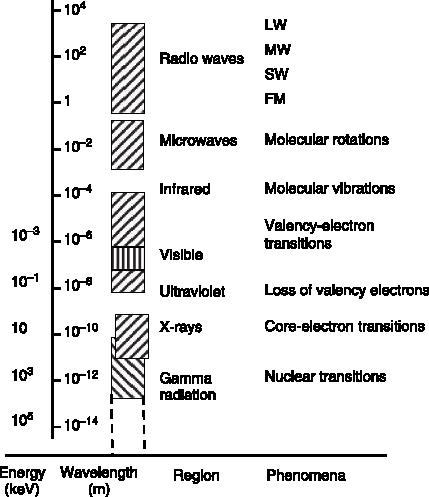
\includegraphics{figures/light_energies.pdf}
    \caption{Grafische Darstellung des elektromagnetischen Spektrums zu unterschiedlichen Wellenlängen \cite{gamma}.}
    \label{fig:ems}
\end{figure}

Als Gammastrahlung werden Photonen, also elektromagnetische Strahlung, mit einer Energie zwischen circa $\SI{10}{\kilo\eV}$ und $\SI{10000}{\kilo\eV}$ bezeichnet.
Anders als bei $\alpha$- und $\beta$-Strahlung handelt es sich bei $\gamma$-Strahlung um ungeladene Strahlung mit hoher Reichweite und Eindringtiefe.
Gammastrahlung kann durch unterschiedliche Prozesse, darunter z.B. der Zerfall von Positronen und anderen Teilchen oder Bremsstrahlung entstehen.
Da hier aber das Gammaspektrum von Atomkernen betrachtet werden soll, sind insbesondere Photonen, die in Kernzerfällen entstehen, wichtig.
Findet in einem Kern ein $\alpha$- oder $\beta$-Zerfall statt, verbleibt der Kern oft in einem angeregten und instabilen Energiezustand.
Dort fällt er nach einer bestimmten Zeit (meistens in der Größenordnung einiger $10^{-12}\, \si{\second}$) in einen stabilen niederenergetischen Zustand zurück.
Die Energiedifferenz zwischen den beiden Zuständen wird in Form eines Photons abgestrahlt \cite{gamma}. \\

Diese Photonen verlassen den Kern und können auf verschiedene Weise mit der umliegenden Materie interagieren.

\subsubsection{Photoeffekt}

Beim Photoeffekt wird das emittierte Photon von einem Elektron absorbiert.
Ist die Photonenenergie höher als die Bindungsenergie $E_\text{B}$, die das Elektron an den Kern bindet, wird es mit der Energie $E_\text{e} = E_\gamma - E_\text{B}$
aus der Atomhülle emittiert.
Das freie Elektron gibt seine Energie durch die Emission weiterer Photonen oder Kollisionen mit anderen Elektronen ab.
Da das Photon vollständig absorbiert wird kann dieser Prozess zur Energiebestimmung genutzt werden.

\subsubsection{Comptoneffekt}

Anders als beim Photoeffekt beschreibt der Comptoneffekt, auch Comptonstreuung, wie in \autoref{fig:comptonscattering} die Streuung eines Photons an einem Elektron.

\begin{figure}
    \centering
    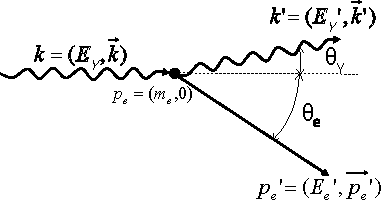
\includegraphics{figures/compton.pdf}
    \caption{Schematische Darstellung der Streuung eines Photons an einem Elektron \cite{Teilchendetektoren}.}
    \label{fig:comptonscattering}
\end{figure}

Bei der Streuung wird abhängig vom Streuwinkel ein Energiebruchteil
\begin{equation}
    E_{\gamma'} = E_\gamma \frac{1}{1 + \varepsilon (1 - \cos\theta)}
    \label{eq:Egammaprime}
\end{equation}
an das Elektron übertragen. \\
Mit $\varepsilon = \frac{E_\gamma}{m_\text{e} c^2}$ ist die Elektronenenergie nach der Streuung durch
\begin{equation}
    E_\text{e} = E_\gamma -E_{\gamma'} = E_\gamma (1 - \frac{1}{1 + \varepsilon (1 - \cos\theta)}) 
    \label{eq:elektronenenergie}
\end{equation}
gegeben. \\

Die Klein-Nishima-Gleichung liefert dann den differentiellen Wirkungsquerschnitt
\begin{equation}
    \frac{\text{d}\sigma_C}{\text{d}\Omega} = \frac{r_\text{e}^2}{2 (1 + \varepsilon (1 - \cos\theta))^2} 
                                              \left(1 + \cos^2\theta + \frac{\varepsilon^2 (1 - \cos\theta)^2}{1 + \varepsilon (1 - \cos\theta)} \right)
                                              \label{eq:dcrossomega}
\end{equation}
pro Raumwinkel und freiem Elektron, der sich mit $t = \frac{E_\text{e}}{E_\gamma}$ auch als Ableitung nach der Elektronenenergie darstellen lässt, sodass
\begin{equation}
    \frac{\text{d}\sigma_C}{\text{d}E_\text{e}} = \frac{\pi r^2_\text{e}}{m_\text{e} c^2 \varepsilon^2} 
                                                  \left(2 + \frac{t^2}{\varepsilon^2 (1-t)^2} + \frac{t}{1-t} \left(t - \frac{2}{\varepsilon}\right)\right)
    \label{eq:Comptonkontinuum}
\end{equation}
ebenfalls den differentiellen Wirkungsquerschnitt beschreibt \cite{Teilchendetektoren}.

\subsubsection{Paarerzeugung}

Da der hier verwendete Detektor eine obere Energieschranke von etwa $\SI{5}{\mega\eV}$ aufweist ist die Paarerzeugung der höchstenergetische relevante Prozess.
Im Coulombfeld eines Atomkerns produziert das Photon ein $e^+ e^-$-Paar, von denen das Positron in den meisten Fällen in kurzer Zeit mit einem Hüllenelektron annihiliert,
sodass das Elektron detektiert werden kann.
Da hier ein Paar mit einer Ruhemasse von etwa $\SI{1000}{\kilo\eV}$ erzeugt wird ist auch die Energiegrenze dieses Prozesses ähnlich hoch.


\subsection{Absorptionskoeffizient}

Um zu beschreiben, wie tief die enstandenen Gammaphotonen in ein Medium eindringen können, ist der Absorptionskoeffizient $\mu$ hilfreich.
Wie in \autoref{fig:Absorptionskoeffizient} zu erkennen ist, tragen bei unterschiedlichen Energien die bereits erläuterten Prozesse zur Gesamtextinktion bei.

\begin{figure}[H]
    \centering
    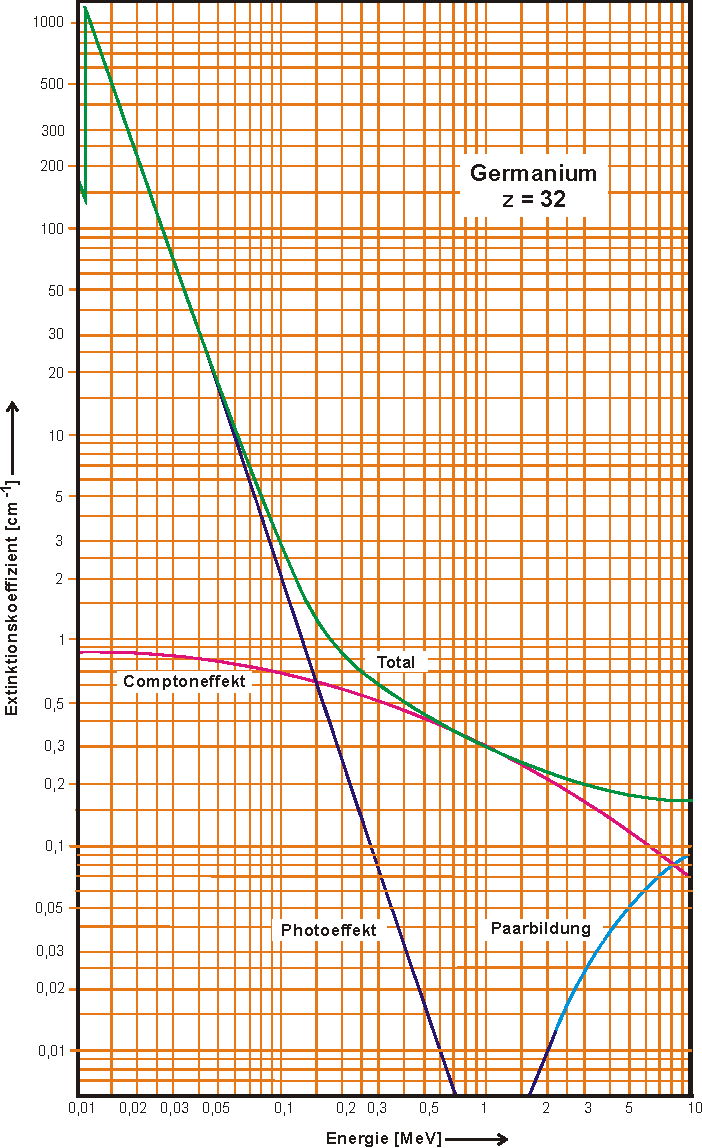
\includegraphics{figures/extinction_coefficient.pdf}
    \caption{Gesamter Absorptionskoeffizient $\mu$ sowie Einzelbeiträge aus dem Photo- und Comptoneffekt sowie der Paarerzeugung am Beispiel von Germanium-32 \cite{ap704}.} 
    \label{fig:Absorptionskoeffizient}   
\end{figure}

Wie bereits in der Beschreibung der Paarbildung angerissen ist diese nur für die höchsten Energien der dominierende Prozess.
Im Bereich unterhalb etwa $\SI{8}{\mega\eV}$ dominieren Photo- und Comptoneffekt.
Der Photoeffekt trägt unterhalb etwa $\SI{0.15}{\mega\eV}$ stärker als der Comptoneffekt bei. \\

Kenntnis über den Absorptionskoeffizienten eines Mediums erlaubt es, 
die Absorptionswahrscheinlichkeit von Photonen unterschiedlicher Energie in einem Detektor der Länge $l$ über
\begin{equation}
    P(\mu) = 1 - \text{e}^{-l \mu} \,,
    \label{eq:Absorptionswahrscheinlichkeit}
\end{equation}
zu beschreiben.

\subsection{Der Germaniumdetektor}

Mit einer Bandlücke von nur $\SI{0,7}{\eV}$ und einer mittleren Energie zur Erzeugung eines Elektron-Loch-Paares von $\SI{2,96}{\eV}$ verfügt Germanium gegenüber anderen
konventionellen Detektormaterialen, darunter z.B. Silizium, über eine bessere Energieauflösung \cite{Teilchendetektoren}. \\
In Germaniumdetektoren sind sowohl p- als auch n-dotierte, also mit einem Ladungsmangel bzw. Ladungsüberfluss versehene, 
Halbleiter verbaut.
An der Grenzfläche zwischen den beiden dotierten Halbleitern kommt entsteht eine Verarmungszone. 
Löst ein eintreffendes Photon ein Elektron-Loch-Paar in dieser Verarmungszone,
rekombinieren Elektron und Loch nicht wie im restlichen Detektor, sondern wandern in Richtung der p- bzw. n-dotierten Halbleiter.
Zusammen mit einer äußeren Biasspannung wandern Elektron und Loch vollends zu ihren korrespondierenden Elektroden und können dort als Strom gemessen werden.
Die Anzahl gelöster Elektron-Loch-Paare und damit auch der gemessene Strom ist proportional zur Photonenenergie.
Dennoch ist die Energie der Gammaphotonen zu hoch, um effizient von Detektoren mit konventionellen Verarmungszonen detektiert werden zu können.
Es ist möglich, hochreine Germaniumkristalle mit einer Verarmungszone zu wachsen, die statt einigen $\si{\milli\meter}$ einige Zentimeter dick ist.
Alternativ kann das Germanium auch mit Lithium dotiert werden, um eine größere Verarmungszone zu erreichen.
In beiden Fällen muss der Detektor gekühlt werden, sei es im Fall des hochreinen Germaniums nur, um das thermische Rauschen,
das aufgrund der kleinen Bandlücke von Germanium verstärkt auftritt möglichst stark zu unterdrücken. \\

Doch auch mit erhöhter Verarmungszonenbreite ist die Effizienz bei der Detektion von $\gamma$-Strahlung vergleichsweise niedrig.
Bei einer Messzeit $t$ für einen Detektor mit Radius $r$ und Winkelabdeckung
\begin{equation*}
    \Omega = 2 \pi \left(1 - \frac{a}{\sqrt{a^2 + r^2}}\right) \,,
\end{equation*}
der eine Quelle der Aktivität
\begin{equation*}
    A(t) = A_0 \exp \left(-\frac{\ln(2)}{T_{1/2}} t \right)
\end{equation*}
im Abstand $a$ misst, beträgt die Detektionseffizienz
\begin{equation}
    Q = \frac{4 \, \pi \, Z}{A \, W \, t \, \Omega} \,.
\end{equation}
Dabei ist $W$ die Emissionswahrscheinlichkeit der untersuchten Emissionslinie \cite{gamma}.

\subsection{Spektrum eines monochromatischen Gammastrahlers}

Nach dem Sammeln aller nötigen Grundlagen wird jetzt auf das Spektrum eines monochromatischen Gammastrahlers, wie in \autoref{fig:gammaspektrum} dargestellt, eingegangen.

\begin{figure}[H]
    \centering
    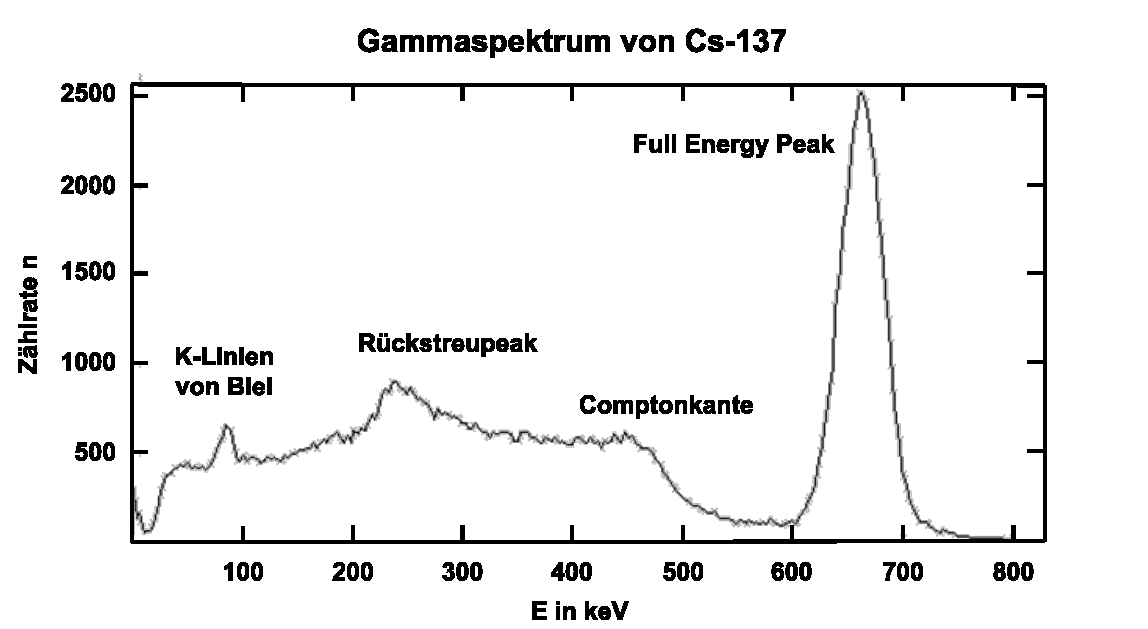
\includegraphics{figures/Gammaspektrum.pdf}
    \caption{Monochromatisches Gammasprektrum am Beispiel von Cs-137. Hervorgehoben sind der Full Energy Peak, auch Photopeak,
    der Rückstreupeak und die Comptonkante sowie die K-Linien von Blei, die hier nicht relevant sind \cite{gammaspektrum}.}
    \label{fig:gammaspektrum}
\end{figure}

Markant ist insbesondere der sogenannte Photopeak bei der vollen Photonenergie $E_\gamma$.
Dort deponiert das Photon seine gesamte Energie über den Photoeffekt.
Das Comptonkontinuum, die Comptonkante sowie der Rückstreupeak entstehen durch den Comptoneffekt.
Hier wird, abhängig vom kontinuierlichen Winkel $\theta$, nur ein Bruchteil der Photonenenergie deponiert.
Die beiden Grenzfälle $\theta = 0$ sowie $\theta = \pi$ liefern in \eqref{eq:elektronenenergie} den Energieübertrag an das Elektron und damit an den Detektor.
Für einen Streuwinkel von $\theta = 0$ findet kein Energieübertrag statt, es gilt also $E_\text{e}(0) = 0$.
Der maximale Energieübertrag, also der Energieübertrag an der Comptonkante, berechnet sich dann zu
\begin{equation}
    E_\text{Comptonkante} = E_\text{e} (\theta = \pi) = E_\gamma \frac{2 \varepsilon}{1 + 2 \varepsilon} \,.
    \label{eq:Comptonpeak}
\end{equation}

Der Rückstreupeak entsteht durch Photonen, die an der Hülle des Detektors zurück in den Detektor gestreut werden.
Sie besitzen nach \eqref{eq:Egammaprime} mit $\theta = \pi$ näherungsweise eine Energie von
\begin{equation}
    E_\text{Rückstreupeak} = E_\gamma \frac{1}{1 + 2 \varepsilon} \,.
    \label{eq:Rückstreupeak}
\end{equation}







